%%%%%%%%%%%%%%%%%%%%%%%%%%%%%%%%%%%%%%%%%%%%%%%%%%%%%%%%%%%%%%%%%%%%%%%%%%%

\section{Distributed Memory Systems}

\begin{frame}\frametitle{Distributed Memory Systems}



\begin{itemize}
\item Current parallel systems have various architectures.
\item \textbf{MIMD:} shared memory and \textbf{distributed memory systems}
\item Why not use share-memory systems and programming models always? 
\begin{itemize}
\item System scaling is limited by the bus interconnect!
\item Distributed systems are better suited for problems requiring vast amount of data or computation.
\end{itemize}
\end{itemize}

\begin{figure}
\centering
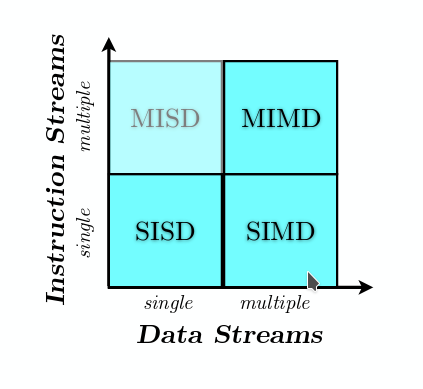
\includegraphics[width=0.35\textwidth]{img/Flynn.png}
\end{figure} 

  
\end{frame}

\begin{frame}\frametitle{Distributed Memory Systems}



\begin{itemize}
\item Each processor has its own private memory.
\item A network connects all the processors.
\item Processors can be asynchronous, programmer must impose synchronization. 
\end{itemize}

\begin{figure}
\centering
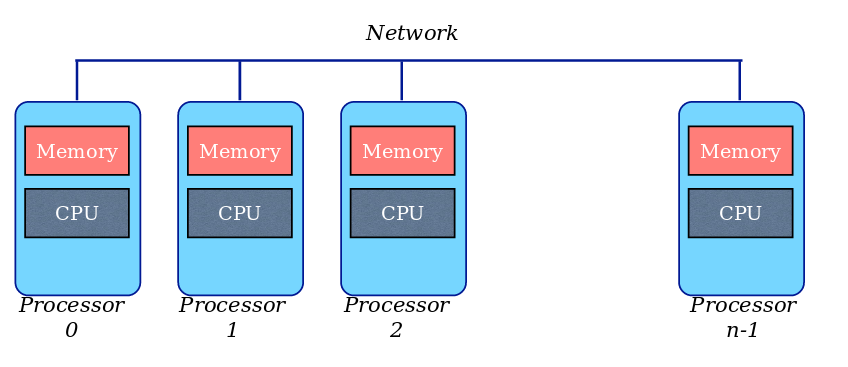
\includegraphics[width=0.8\textwidth]{img/distributeArchitecture.png}
\end{figure} 

  
\end{frame}

\begin{frame}\frametitle{Distributed Memory Systems - Top500}

\begin{figure}
\centering
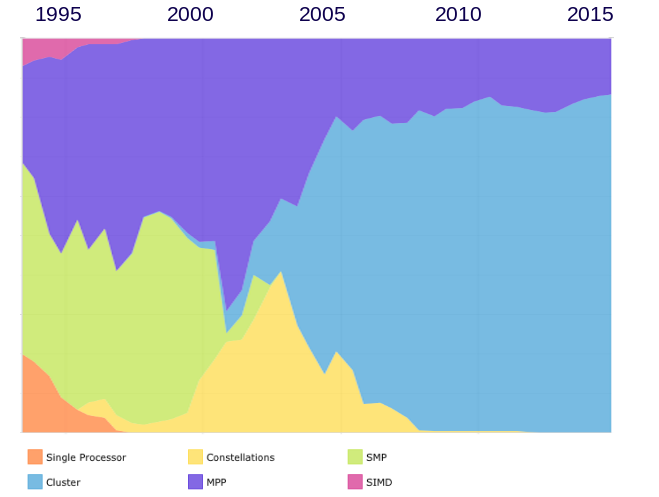
\includegraphics[width=0.65\textwidth]{img/top500.png}
\end{figure} 

  
\end{frame}



%%%%%%%%%%%%%%%%%%%%%%%%%%%%%%%%%%%%%%%%%%%%%%%%%%%%%%%%%%%%%%%%%%%%%%%%%%%

\section{Parallel Programming Model}
\begin{frame}\frametitle{What is a Parallel Programming Model?}

\vspace{5mm}
\begin{itemize}
\item {\Large An abstract machine on which parallel programs will execute.}
\vspace{5mm}
\item {\Large Components:}
\begin{itemize}
\item {\large Execution model: how codes gets executed.}
\vspace{2mm}
\item {\large Memory model: how data moves between memory hierarchy.}
\end{itemize}
\vspace{5mm}
\item {\Large Most parallel systems expose multiple parallel programming models.}
\end{itemize}

\end{frame}

\begin{frame}\frametitle{Desirable Features}

\vspace{5mm}
\begin{itemize}
\item {\Large \textit{Performant:} extracts as much performance as possible from the underlying hardware.}
\vspace{5mm}
\item {\Large \textit{Productive:} expresses abstract algorithms easily.}
\vspace{5mm}
\item {\Large \textit{Portable:} can be used on any computer.}
\vspace{5mm}
\item {\Large \textit{Expressive:} allows a broad range of algorithms.}
\vspace{5mm}
\item {\Large \textit{Scalable:} the general structure of the code persists as more hardware is used.}
\end{itemize}

\end{frame}

\begin{frame}\frametitle{Implementation}

\vspace{5mm}
\begin{itemize}
\item {\Large \textit{Library:}}
\begin{itemize}
\item {\large An API of function calls.}
\vspace{1mm}
\item {\large Library gets linked with the executable; multiple languages.}
\end{itemize}
\vspace{5mm}
\item {\Large \textit{Programming Language Extension:} }
\begin{itemize}
\item {\large Additional constructs for parallelism.}
\vspace{1mm}
\item {\large Compiler support for translation.}
\end{itemize}
\vspace{5mm}
\item {\Large \textit{New Programming Language:}}
\begin{itemize}
\item {\large Design of new language grammar.}
\vspace{1mm}
\item {\large Flexibility to include features.}
\end{itemize}
\end{itemize}

\end{frame}

{
\usebackgroundtemplate{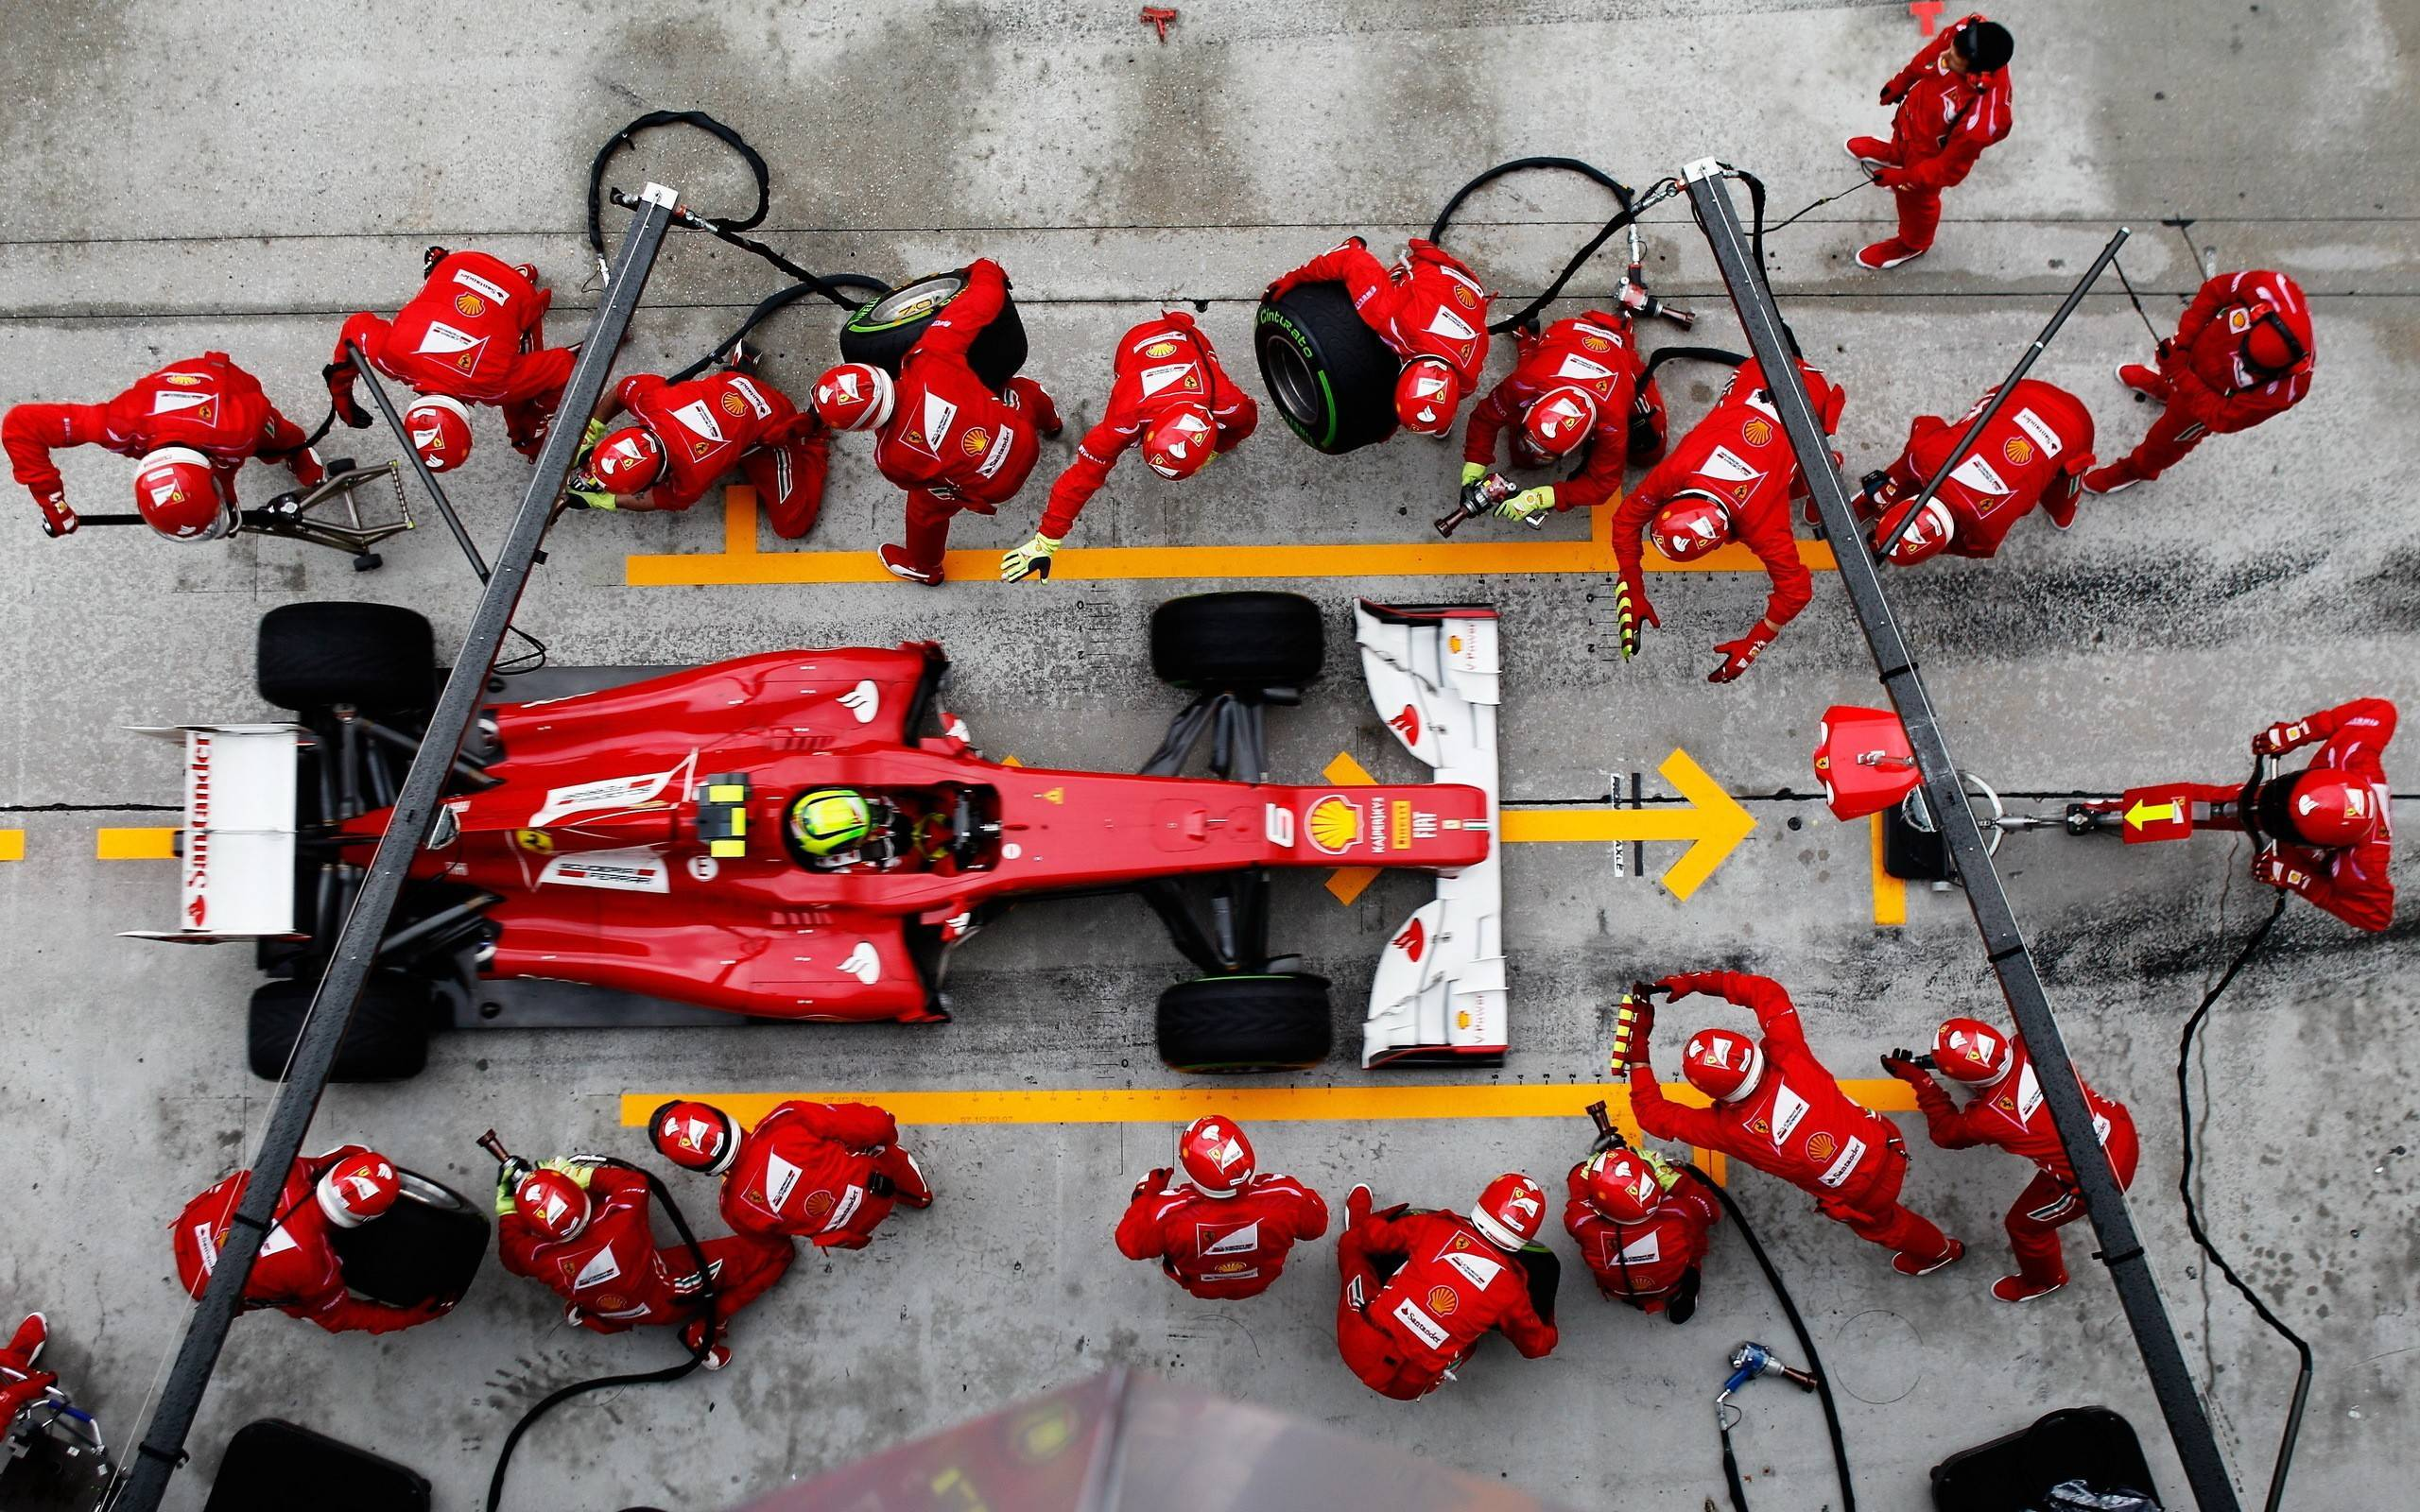
\includegraphics[width=1\paperwidth]{img/formulaOne.jpg}}
\begin{frame}[plain]
\end{frame}
}

\begin{frame}\frametitle{Message-Passing Paradigm}

\vspace{5mm}
\begin{itemize}
\item {\Large A parallel program is decomposed into processes, called ranks.}
\vspace{3mm}
\item {\Large Each rank holds a portion of the program’s data into its private memory.}
\vspace{3mm}
\item {\Large Communication among ranks is made explicit through messages.}
\vspace{3mm}
\item {\Large Channels honor first-in-first-out (FIFO) ordering.}
\end{itemize}

\end{frame}

\begin{frame}{Bulk Synchronous Parallelism}

\begin{columns}
\begin{column}{0.5\textwidth}
  \begin{itemize}
  \item Bridging model developed by Leslie Valiant 1980.
  \item Model components:
      \begin{itemize}
      \item Processors
      \item Network
      \item Synchronization hardware
      \end{itemize}
  \item Computation proceeds by executing \textit{supersteps}:
      \begin{itemize}
      \item Concurrent computation
      \item Communication
      \item Barrier Synchronization
      \end{itemize}
  \item Concurrency level expands and shrinks. 
  \end{itemize}
\end{column}
\begin{column}{0.5\textwidth}  %%<--- here
    \begin{center}
     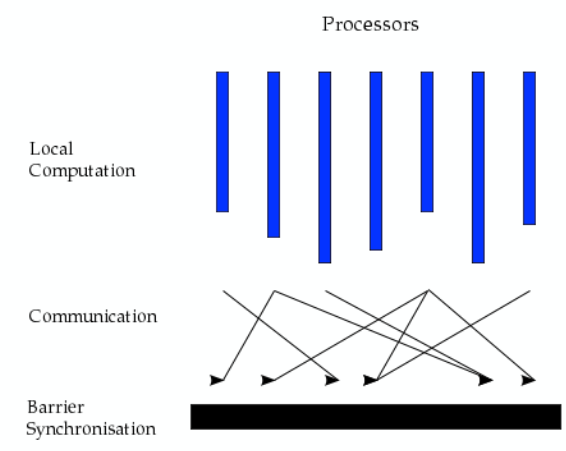
\includegraphics[width=0.85\textwidth]{img/BSP.png}
     \end{center}
\end{column}
\end{columns}
    
\end{frame}

\begin{frame}\frametitle{Single-Program Multiple-Data (SPMD)}

\vspace{5mm}
\begin{itemize}
\item {\Large All processes run the same program, each accesses a different portion of data.}
\vspace{3mm}
\item {\Large All processes are launched simultaneously.}
\vspace{3mm}
\item {\Large Communication:}
\begin{itemize}
\item {\large Point-to-point messages.}
\vspace{1mm}
\item {\large Collective communication operations.}
\vspace{1mm}
\item {\large One-sided communication. }
\end{itemize}
\end{itemize}

\end{frame}

\begin{frame}\frametitle{Features of Message Passing}

\vspace{5mm}
\begin{itemize}
\item {\Large \textit{Simplicity: } the basics of the paradigm are traditional communication operations.}
\vspace{5mm}
\item {\Large \textit{Generality:} can be implemented on most parallel architectures.}
\vspace{5mm}
\item {\Large \textit{Performance:} the implementation can match the underlying hardware.}
\vspace{5mm}
\item {\Large \textit{Scalability:} the same program can be deployed on larger systems.}
\end{itemize}

\end{frame}


%%%%%%%%%%%%%%%%%%%%%%%%%%%%%%%%%%%%%%%%%%%%%%%%%%%%%%%%%%%%%%%%%%%%%%%%%%%

\section{Message Passing Interface}
\begin{frame}{Message Passing Interface}
    \begin{itemize}
        \item Message-passing library interface specification.
        \vspace{2mm}
        \item Standard for operations in message passing.
        \vspace{2mm}
        \item Operations are expressed as functions, subroutines or methods depending on the language and implementation. 
        \vspace{2mm}
        \item Goals: 
        \begin{itemize}
        \item Allow efficient communication.
        \vspace{1mm}
        \item Allow overlap of communication and computation.
        \vspace{1mm}
        \item Allow for implementations that can be used in heterogeneous environments. 
        \end{itemize}
         \vspace{1mm}
        \item Implementations:
        \begin{itemize}
        \item Open-source: MPICH, OpenMPI.
        \vspace{1mm}
        \item Proprietary: Cray, IBM, Intel.
        \end{itemize}
         \vspace{1mm}
        \item Languages:
        \begin{itemize}
        \item C/C++, Fortran, Python, Perl, Ruby, R, Java, CL, Haskell.
        \end{itemize}
        
    \end{itemize}
\end{frame}

\begin{frame}{MPI Background}
    \begin{itemize}
    \item Numerous message passing systems existed before MPI.
      \vspace{2mm}
    \item MPI forum (academia and industry) was created in 1992.
      \vspace{2mm}
    \begin{itemize}
    \item MPI-1(1993): focused mainly on point-to-point communications.
    \vspace{1mm}
    \item MPI-2 (1997): included one-sided communications, collective communications and aspects of parallel I/O. 
    \vspace{1mm}
    \item MPI-3 (2012): major update to the standard. Included non-blocking collectives and new one-sided operations.
    \vspace{1mm}
    \item MPI-3.1 (2015): minor revisions to the third version of the standard.  
    \end{itemize}
    \vspace{2mm}
    \item Standard provides portability and ease of use!
    \vspace{2mm}
    \item There is no automatic sequential-equivalent to an MPI program.
    
        
    \end{itemize}
\end{frame}

\begin{frame}{MPI Ranks}
    \begin{itemize}
    \item Ranks have private memory.
    \vspace{2mm}
    \item Each rank has a unique identification number.
    \vspace{2mm}
    \item Ranks are numbered sequentially: [0,n-1].
    \vspace{2mm}
    \item There is no automatic sequential-equivalent to an MPI program.
    \end{itemize}
    
    \begin{figure}
    \centering
    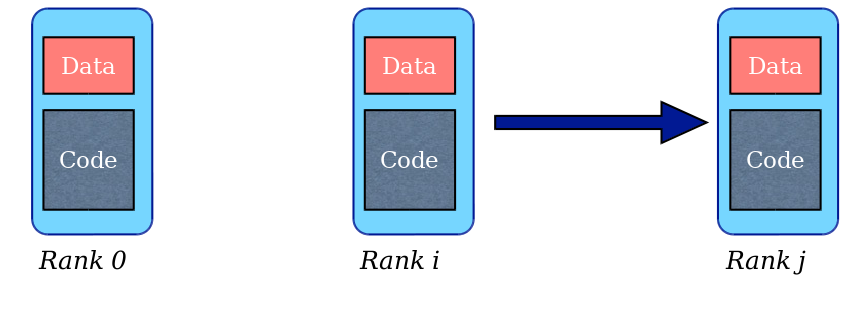
\includegraphics[width=0.7\textwidth]{img/mpiRanks.png}
    \end{figure} 
    
\end{frame}

\begin{frame}{MPI Communicators}
    \begin{itemize}
    \item Groups of ranks among which ranks can communicate.
    \vspace{2mm}
    \item COMM\_WORLD is a communicator including all ranks in the system.
    \vspace{2mm}
    \end{itemize}
    
    \begin{figure}
    \centering
    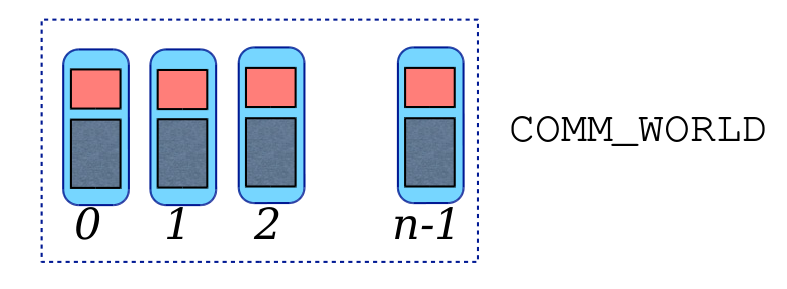
\includegraphics[width=0.7\textwidth]{img/communicators.png}
    \end{figure} 
    
\end{frame}

\begin{frame}[fragile]{MPI Primer}


\begin{itemize}
\item Initialization:
\end{itemize}
    \begin{verbatim}
    int MPI_Init(int *argc, char ***argv)
    \end{verbatim}
    \vspace{-3mm}
\begin{itemize}
\item Get communicator size:
\end{itemize}
    \begin{verbatim}
    int MPI_Comm_size(MPI_Comm comm, int *size)
    \end{verbatim}
    \vspace{-3mm}
\begin{itemize}
\item Get rank number:
\end{itemize}
    \begin{verbatim}
    int MPI_Comm_rank(MPI_Comm comm, int *rank)
    \end{verbatim}
    \vspace{-3mm}
\begin{itemize}
\item Finalization:
\end{itemize}
    \begin{verbatim}
    int MPI_Finalize(void)
    \end{verbatim}

    
\end{frame}

\begin{frame}[fragile]{MPI Hello World}

\scriptsize\begin{verbatim}
#include <mpi.h>  //Contains prototypes of MPI functions, macro and type definitions...
#include <stdio.h>
#include <stdlib.h>

// Main routine
int main (int argc, char *argv[]){
    int rank,size,length;
    char name[25];

    // initialize MPI
    MPI_Init(&argc, &argv);
    MPI_Comm_rank(MPI_COMM_WORLD, &rank);
    MPI_Comm_size(MPI_COMM_WORLD, &size);
    MPI_Get_processor_name(name, &length);
    printf( "Hello world from rank %d of %d on host %s\n", rank, size,name);

    // finalize MPI
    MPI_Finalize();
    return 0;
}

\end{verbatim}
\normalsize
   
 
    
\end{frame}

\begin{frame}[fragile]{Kabré: running MPI code}

\begin{itemize}
\item Compile application on login nodes using mpicc (wrapper for the C compiler).
\end{itemize}

\small\begin{verbatim}

        mpicc hello.c -o hello
\end{verbatim}
\normalsize

\begin{itemize}
\item To execute MPI applications on Kabré use a PBS script.
\end{itemize}
\small\begin{verbatim}

        #PBS -N HelloMPI
        #PBS -q phi-n2h72
        #PBS -l nodes=2:ppn=4
        #PBS -l walltime=0:30:00
        cd $PBS_O_WORKDIR
        module load mpich
        mpiexec -n 8 ./hello
        
\end{verbatim}
\normalsize
 \vspace{-2mm}
\begin{itemize}
\item Submit the job using queues.
\end{itemize}
 
\small\begin{verbatim}

        qsub hello.pbs
        
\end{verbatim}
\normalsize
\end{frame}

%%%%%%%%%%%%%%%%%%%%%%%%%%%%%%%%%%%%%%%%%%%%%%%%%%%%%%%%%%%%%%%%%%%%%%%%%%%

\section{Point-to-point Communications}

\subsection{Blocking Point-to-point Communications}
\begin{frame}[fragile]{Blocking Point-to-point Communications}
    \begin{itemize}
        \item Instructions to send a message from one source rank to a destination rank: 
    \end{itemize}
\vspace{-2mm}
\scriptsize\begin{verbatim}
            int MPI_Send(void *buf, int count, MPI_Datatype datatype,
                        int dest, int tag, MPI_Comm comm)
            
            int MPI_Recv(void *buf, int count, MPI_Datatype datatype, 
                 int  source, int tag, MPI_Comm comm, MPI_Status *status)
\end{verbatim}
\normalsize
\vspace{-2mm}
\begin{figure}
    \centering
    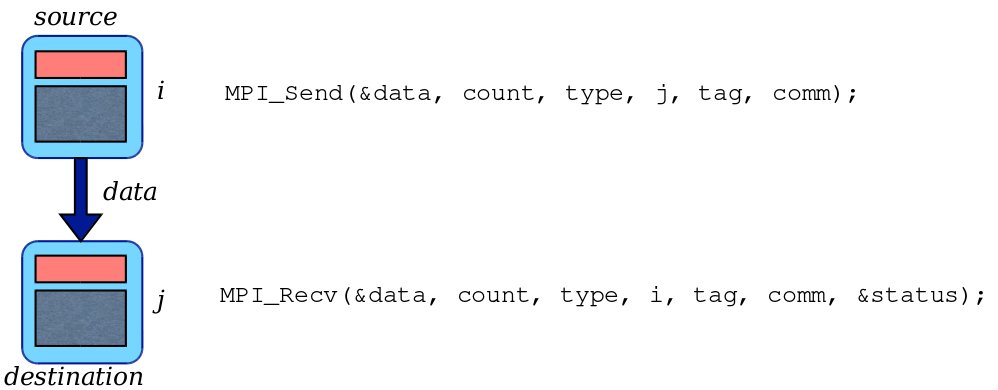
\includegraphics[width=0.5\textwidth]{img/pointpoint.png}
\end{figure} 
\vspace{-2mm}
\begin{alertblock}{Safe communications}
If a send is not paired with a matching receive then the
code will have a \textbf{deadlock}.
\end{alertblock}


\end{frame}

\begin{frame}[fragile]{MPI Message Data}
    \begin{itemize}
        \item Buffer specified by the  communication operations consists of:
            \begin{itemize}
            \item \textbf{count}: amount of succesive entries of the type specified. 
            \item \textbf{datatype}: corresponds to the basic datatypes of the host language.
            \end{itemize}
    \end{itemize}


\begin{center}
 \scriptsize\begin{tabular}{||c c||} 
 \hline
 MPI datatype & C datatype \\ [0.5ex] 
 \hline\hline
 MPI\_CHAR & signed char\\ 
 \hline
 MPI\_DOUBLE & double\\
 \hline
 MPI\_FLOAT & float  \\
 \hline
 MPI\_INT & integer  \\
 \hline
 MPI\_LONG & long  \\
 \hline
 MPI\_BYTE &  8 binary digits \\
 \hline
 MPI\_PACKED & \\ [1ex] 
 \hline
\end{tabular}
\normalsize
\end{center}

\begin{itemize}
        \item Type matching: the type specified by the send operation has to match the type specified by the
                receive operation.
        \item By using MPI derived types, more complex messages can be sent (values with different datatypes or  noncontiguous data). 
\end{itemize}
\end{frame}

\begin{frame}[fragile]{MPI Message Envelope}
\vspace{5mm}
    \begin{itemize}
        \item Messages carry information that helps distinguish them and selectively receive data:
            \begin{itemize}
            \item \textbf{source}
            \vspace{1mm}
            \item \textbf{destination} 
            \vspace{1mm}
            \item \textbf{tag}: identifier to filter or order received messages.  
            \vspace{1mm}
            \item \textbf{communicator}: communication context for an operation. Messages are always received within the context they were sent, and messages sent in different contexts
                    do not interfere.
            \end{itemize}
        \item A message is received by a receive operation only if its envelope matches the source, tag and communicator values specified in the operation. 
        \item MPI provides certain wild card values: MPI\_ANY\_SOURCE and MPI\_ANY\_TAG.
    \end{itemize}
\end{frame}

\begin{frame}[fragile]{Send-Receive Example}

\tiny\begin{verbatim}
#include <mpi.h>
#include <stdio.h>

int main(int argc, char ** argv)
{
    int rank, data[3];
    MPI_Init(&argc, &argv);
    MPI_Comm_rank(MPI_COMM_WORLD, &rank);
    
    if (rank == 0) {
        data[0] = 0; data[1] = 10; data[2] = 20;
        MPI_Send(data, 3, MPI_INT, 1, 0, MPI_COMM_WORLD);
    }
    
    else if (rank == 1) {
        data[0] = -1; data[1] = -1; data[2] = -1;
        printf("[%d] before receiving: %d,%d,%d\n", rank, data[0], data[1], data[2]);
        
        MPI_Recv(data, 3, MPI_INT, 0, 0, MPI_COMM_WORLD, MPI_STATUS_IGNORE);
        
        printf("[%d] after receiving: %d,%d,%d\n", rank, data[0], data[1], data[2]);
    }
    
    MPI_Finalize();
    return 0;
    
}
\end{verbatim}
\normalsize
\end{frame}

\begin{frame}[fragile]{MPI under the hood}

\begin{itemize}
\item MPI implementation must be able to deal with storing data when two or more processes or ranks are out of sync. 
\item A system buffer area is reserved to hold data in transit.
\end{itemize}

\begin{figure}
    \centering
    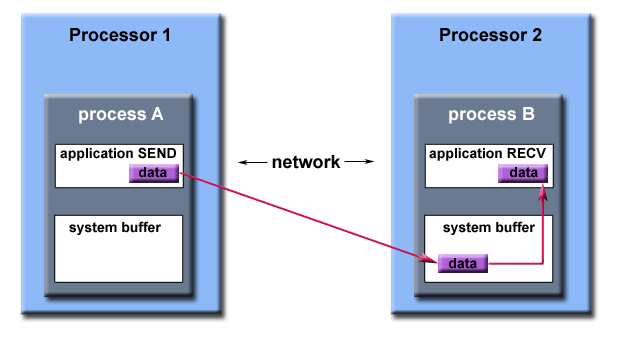
\includegraphics[width=0.65\textwidth]{img/MPIBuffering.png}
\end{figure} 


\end{frame}

\begin{frame}[fragile]{Communication modes}

\begin{itemize}
\item \textbf{Blocking mode} (standard): send operation does not return until the message data and envelope have been safely stored away and the sender is free to modify the buffer. 
\end{itemize}

\small\begin{verbatim}

 int MPI_Send(void *buf, int count, MPI_Datatype datatype, int dest,
 int tag, MPI_Comm comm)

\end{verbatim}
\normalsize


\begin{itemize}
\item \textbf{Buffered mode}: if a send is executed and no matching receive is posted, MPI buffers the outgoing message  to allow the send call to complete. Available buffer space is controlled
by the user.
\end{itemize}

\small\begin{verbatim}

int MPI_Bsend(const void* buf, int count, MPI_Datatype datatype, int dest,
int tag, MPI_Comm comm)

\end{verbatim}
\normalsize

\end{frame}

\begin{frame}[fragile]{Communication modes}

\begin{itemize}
\item \textbf{Synchronous mode}: send operation will complete successfully only if a matching receive is posted, and the receive operation has started to receive the message. 
\end{itemize}
\small\begin{verbatim}

int MPI_Ssend(const void* buf, int count, MPI_Datatype datatype, int dest,
int tag, MPI_Comm comm)
\end{verbatim}
\normalsize
  
\begin{itemize}
\item \textbf{Ready mode}: send operation may be started \textit{only} if a matching receive is already posted. This allows for the removal of a hand-shake operation that is otherwise
required and results in improved performance.
\end{itemize}

\small\begin{verbatim}

int MPI_Rsend(const void* buf, int count, MPI_Datatype datatype, int dest,
int tag, MPI_Comm comm)

\end{verbatim}
\normalsize

\end{frame}


\begin{frame}[fragile]{Send-Receive exercise}

\begin{itemize}
\item Implement a parallel ping-pong in MPI.
    \begin{itemize}
    \item A message carrying an integer counter is exchanged between two ranks.
      \vspace{2mm}
    \item Only rank 1 will increment the counter upon reception.
      \vspace{2mm}
    \item Repeat the process 1000 times.
    \end{itemize}
\end{itemize}

\begin{figure}
    \centering
    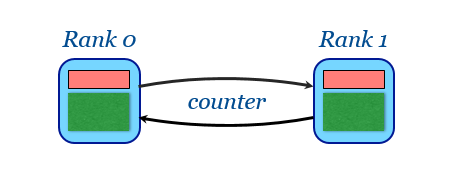
\includegraphics[width=0.6\textwidth]{img/pingpongMPI.png}
\end{figure} 
   
 
    
\end{frame}

\begin{frame}[fragile]{Send-Receive exercise}

\begin{itemize}
\item Implement a parallel MPI program that creates a ring of ranks. 
    \begin{itemize}
    \item Each rank gets a random integer value [0,p]. 
      \vspace{2mm}
    \item The program computes in each rank the sum of all the values by circulating them around the ring.
      \vspace{2mm}
    \end{itemize}
\end{itemize}

\begin{figure}
    \centering
    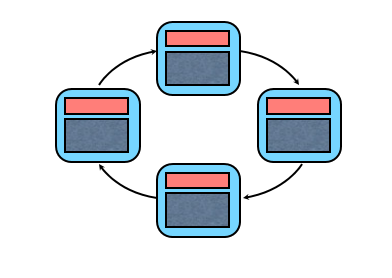
\includegraphics[width=0.5\textwidth]{img/mpiring.png}
\end{figure} 
   
 
    
\end{frame}

\begin{frame}[fragile]{Send-Receive exercise}

\begin{itemize}
\item Using the implemented processors ring: 
    \begin{itemize}
    \item Instead of passing an scalar, try passing an array. 
      \vspace{2mm}
    \item First pass an array of size 100
      \vspace{2mm}
     \item Try setting the size of the array to 100 000. What happens? 
    \end{itemize}
\end{itemize}

\begin{figure}
    \centering
    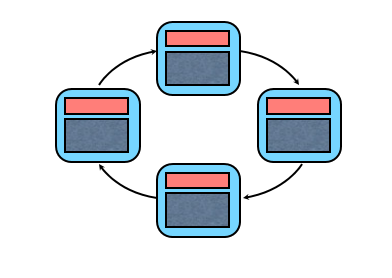
\includegraphics[width=0.5\textwidth]{img/mpiring.png}
\end{figure} 
   
 
    
\end{frame}

\subsection{Nonblocking Point-to-point Communications}
\begin{frame}[fragile]{Problems with blocked communication}
 \vspace{3mm}
\begin{itemize}
\item On rank 0:
\end{itemize}
\small\begin{verbatim}

        MPI_Send( buf, count, type, 1, tag, comm);
        MPI_Recv( buf, count, type, 1, tag, comm, &status);

\end{verbatim}
\normalsize

\begin{itemize}
\item On rank 1: 
\end{itemize}
\small\begin{verbatim}

        MPI_Send( buf, count, type, 0, tag, comm);
        MPI_Recv( buf, count, type, 0, tag, comm, &status);

\end{verbatim}
\normalsize
\vspace{-2mm}
\begin{itemize}
\item A blocking send will only "return" after it is safe to modify the application buffer for reuse.
\item A blocking send can be synchronous which means there is handshaking occurring with the receive task to confirm a safe send. 
\end{itemize}

\end{frame}

\begin{frame}[fragile]{Solving deadlocks}
 \vspace{3mm}
\begin{enumerate}
\item Reorganize send and receive operations.
    \begin{itemize}
    \item Even ranks send first.
    \item Odd ranks receive first. 
    \end{itemize}
     \vspace{3mm}
\item Let MPI take care of the problem:
    \begin{itemize}
    \item MPI\_Sendrecv
    \item MPI\_Sendrecv\_replace
    \end{itemize}
     \vspace{3mm}
\item Use nonblocking communication. 
\end{enumerate}



\end{frame}

\begin{frame}[fragile]{Nonblocking Point-to-point Communications}
    \begin{itemize}
        \item Performance can be boosted by overlapping communication and computation.  
         \vspace{3mm}
        \item Nonblocking operations simply request the MPI implementation to perform the operation when it is able, i.e they do not wait for the operation to complete. 
         \vspace{2mm}
        \item It's unsafe to modify the application buffer (variable) until we verify that the nonblocking operation has been completed. 
        \vspace{3mm}
        \item At least two function calls:
            \begin{enumerate}
            \item Call to start operation.
              \vspace{2mm}
            \item Call to complete the operation. 
            \end{enumerate}
    \end{itemize}
\end{frame}

\begin{frame}[fragile]{Nonblocking Point-to-point Communications}
  \begin{itemize}
  \item Nonblocking operations return "request handles" that can be waited on and queried. 
  \end{itemize}
  \scriptsize\begin{verbatim}

            int MPI_Isend(const void* buf, int count, MPI_Datatype datatype, int dest,
                            int tag, MPI_Comm comm, MPI_Request *request)
                    
            int MPI_Irecv(void* buf, int count, MPI_Datatype datatype, int source,
                            int tag, MPI_Comm comm, MPI_Request *request)
                            
            int MPI_Wait(MPI_Request *request, MPI_Status *status)
    
    \end{verbatim}
    \normalsize
    \begin{itemize}
    \item Completion can also be verified using the nonblocking function MPI\_Test.
    \end{itemize}
     \scriptsize\begin{verbatim}

            int MPI_Test(MPI_Request *request, int *flag, MPI_Status *status)
    
    \end{verbatim}
    \normalsize
\end{frame}

\begin{frame}[fragile]{Nonblocking Point-to-point Communications}
\vspace{-4mm}
\begin{figure}
    \centering
    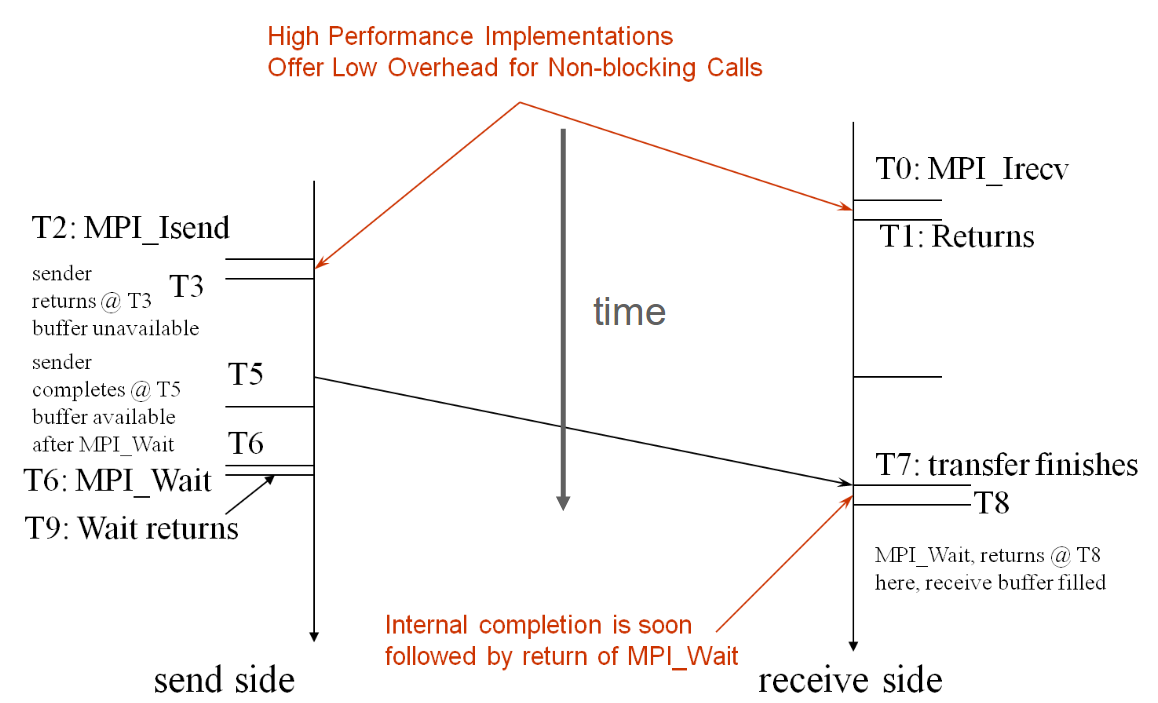
\includegraphics[width=0.8\textwidth]{img/nonblockingMPI.png}
\end{figure} 


\end{frame}

\begin{frame}[fragile]{Isend-Ireceive exercise}

\begin{itemize}
\item Adjust the deadlocked ring, implemented in the blocking communication section, so that it now uses non blocking point-to-point communications: 
    \begin{itemize}
    \vspace{2mm}
    \item First pass an array of size 100
      \vspace{2mm}
    \item Try setting the size of the array to 100 000. What happens now? 
    \end{itemize}
\end{itemize}

\begin{figure}
    \centering
    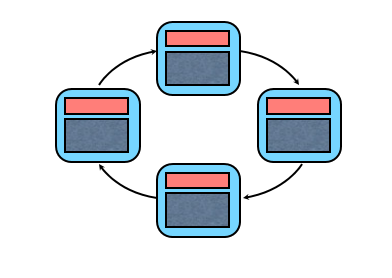
\includegraphics[width=0.5\textwidth]{img/mpiring.png}
\end{figure} 
   
 
    
\end{frame}


%%%%%%%%%%%%%%%%%%%%%%%%%%%%%%%%%%%%%%%%%%%%%%%%%%%%%%%%%%%%%%%%%%%%%%%%%%%

\section{Collective Communication Operations}
\begin{frame}[fragile]{Collective Communication Operations}
    \begin{itemize}
        \item Instructions to exchange data including all the ranks in a communicator.
        \vspace{2mm}
          \item The root rank indicates the source or destination of the operation.
        \vspace{2mm}
        \item All ranks in the communicator must call the collective operation. 
         \vspace{2mm}
        \item Collectives can help implement different communication patterns:
            \begin{itemize}
            \item One-to-many
            \item Many-to-one
            \item Many-to-many
            \end{itemize}
        \item Collectives can serve different purposes:
            \begin{itemize}
            \item Data movement
            \item Collective computation
            \item Synchronization
            \end{itemize}
    \end{itemize}

\end{frame}


\begin{frame}[fragile]{Collective Communication Operations}

\begin{itemize}
\item \textit{Broadcast}: one-to-many
\end{itemize}
\small\begin{verbatim}
           int MPI_Bcast(void *buffer, int count, MPI_Datatype datatype,
              int root, MPI_Comm comm)
\end{verbatim}
\normalsize
    \begin{itemize}
    \item \textit{Reduce}: many to one.
    \end{itemize}
\small\begin{verbatim}
          int MPI_Reduce(const void *sendbuf, void *recvbuf, int count,
                MPI_Datatype datatype, MPI_Op op, int root, MPI_Comm comm)
\end{verbatim}

   \begin{itemize}
    \item \textit{Barrier}: synchronization.
    \end{itemize}
\small\begin{verbatim}
          int MPI_Barrier(MPI_Comm comm)
\end{verbatim}




\end{frame}




\begin{frame}[fragile]{Basic Collectives}
  \vspace{-5mm}
\begin{figure}
    \centering
    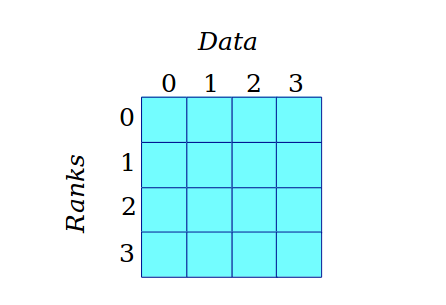
\includegraphics[width=0.4\textwidth]{img/collectivesMPI-1.png}
\end{figure} 
 \vspace{-5mm}

 
\begin{figure}
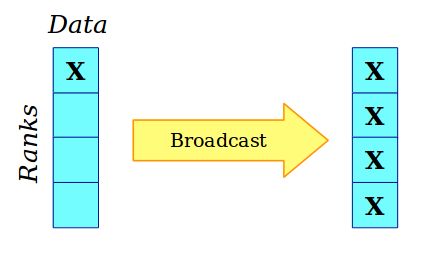
\includegraphics[width=0.35\textwidth]{img/MPI_Broadcast.png} 
\hfill
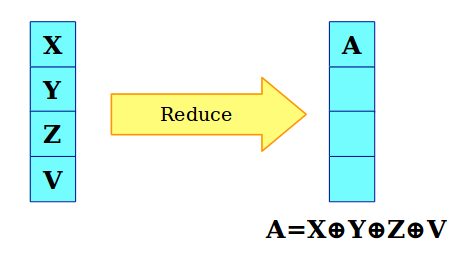
\includegraphics[width=0.35\textwidth]{img/MPI_Reduce.png}

\end{figure}


 

\end{frame}



\begin{frame}[fragile]{Basic Collectives}

\begin{figure}
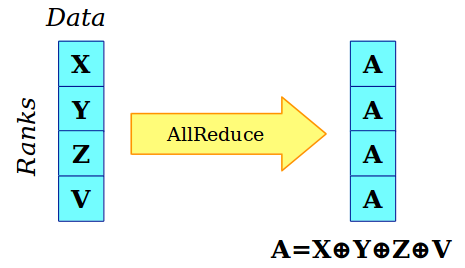
\includegraphics[width=0.4\textwidth]{img/MPI_AllReduce.png} 
\hfill
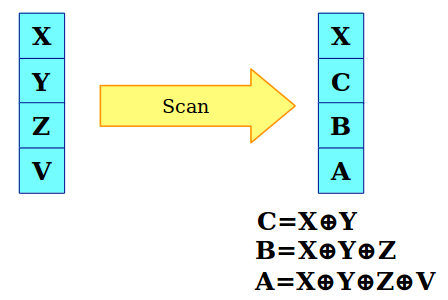
\includegraphics[width=0.4\textwidth]{img/MPI_Scan.png}
\end{figure}

  \vspace{-5mm}
\begin{figure}
    \centering
    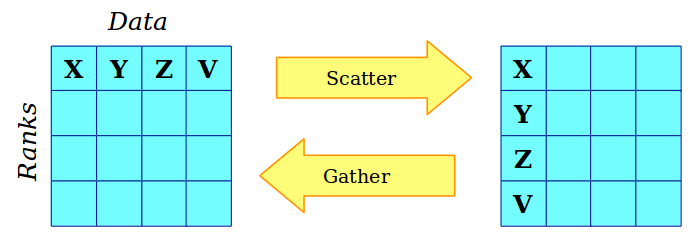
\includegraphics[width=0.5\textwidth]{img/MPI_ScatterGather.png}
\end{figure} 
\end{frame}

\begin{frame}[fragile]{Basic Collectives}

\begin{figure}
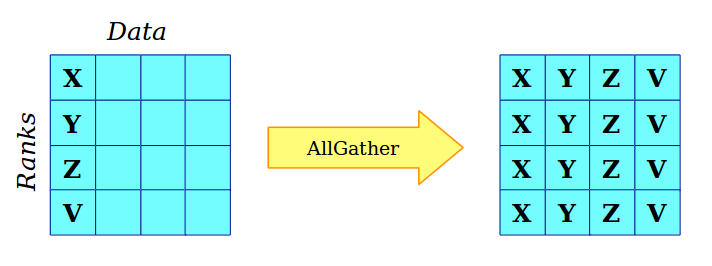
\includegraphics[width=0.6\textwidth]{img/MPI_AllGather.png} 
\end{figure}

  \vspace{-3mm}
  
\begin{figure}
    \centering
    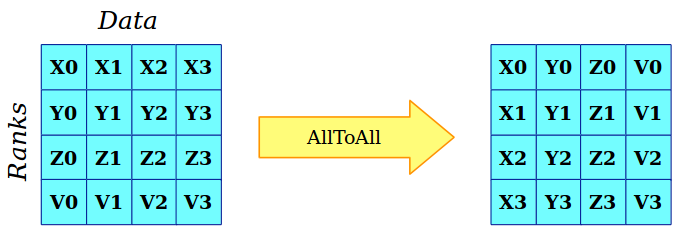
\includegraphics[width=0.6\textwidth]{img/MPI_AlltoAll.png}
\end{figure} 
\end{frame}

\begin{frame}[fragile]{Basic Collectives}
  \vspace{-3mm}
\small\begin{verbatim}
int MPI_Allreduce(const void *sendbuf, void *recvbuf,
    int count, MPI_Datatype datatype, MPI_Op op, MPI_Comm comm)
int MPI_Scan(const void *sendbuf, void *recvbuf, int count, 
    MPI_Datatype datatype, MPI_Op op, MPI_Comm comm)
int MPI_Scatter(const void *sendbuf, int sendcount, 
    MPI_Datatype sendtype, void *recvbuf, int recvcount,
    MPI_Datatype recvtype, int root, MPI_Comm comm)
int MPI_Gather(const void *sendbuf, int sendcount, 
    MPI_Datatype sendtype, void *recvbuf, int recvcount,
    MPI_Datatype recvtype, int root, MPI_Comm comm)
int MPI_Allgather(const void *sendbuf, int sendcount, 
    MPI_Datatype sendtype, void *recvbuf, int recvcount,
    MPI_Datatype recvtype, MPI_Comm comm)
int MPI_Alltoall(const void *sendbuf, int sendcount, 
    MPI_Datatype sendtype, void *recvbuf, int recvcount,
    MPI_Datatype recvtype, MPI_Comm comm)

\end{verbatim}
\normalsize
   

\end{frame}

\begin{frame}[fragile]{Predefined Reduction Operations}

\vspace{5mm}
\begin{center}
 \begin{tabular}{||c c||} 
 \hline
 Name & Meaning \\ [0.5ex] 
 \hline\hline
 MPI\_MAX & maximum  \\ 
 \hline
 MPI\_MIN & minimum \\
 \hline
 MPI\_SUM & sum \\
 \hline
 MPI\_PROD & product \\
 \hline
 MPI\_LOR & logical OR \\
 \hline
 MPI\_LAND & logical AND \\
 \hline
 MPI\_MAXLOC & max value and location \\ [1ex] 
 \hline
\end{tabular}
\end{center}



\end{frame}



\begin{frame}[fragile]{Collectives example: Sequential code}
  \vspace{-3mm}
\small\begin{verbatim}
#include <stdio.h>

int main(int argc, char *argv[]){
        int i, sum, upToVal;
        upToVal = 10000;
        sum = 0;

        for(i=1; i <= upToVal; i++){
                sum = sum +i;
        }
        printf("\nSum is %d\n", sum);
    return 0;
}

\end{verbatim}
\normalsize
   

\end{frame}

\begin{frame}[fragile]{Collectives example: Parallel code}
  \vspace{-3mm}
\scriptsize\begin{verbatim}

#include <stdio.h>
#include "mpi.h"

int main(int argc, char *argv[]){

        int i, sum, sumTotal, upToVal;
        int start, end, size, myRank;

        upToVal = 10000;

        MPI_Init(&argc, &argv);
        MPI_Comm_size(MPI_COMM_WORLD, &size);
        MPI_Comm_rank(MPI_COMM_WORLD, &myRank);

        start = myRank*(upToVal/size)+1;

        if(myRank == (size-1)){
                end = upToVal;
        }else{
              	end = start + (upToVal/size)-1;
        }



\end{verbatim}
\normalsize
   

\end{frame}

\begin{frame}[fragile]{Collectives example: Parallel code}
  \vspace{-3mm}
\scriptsize\begin{verbatim}

        sum = 0;
        sumTotal = 0;

        for(i=start; i <= end; i++){
                sum = sum +i;
        }

	        MPI_Reduce(&sum, &sumTotal, 1, MPI_INT, MPI_SUM, 0, MPI_COMM_WORLD);

        printf("\nRank: %d, local sum: %d, total sum: %d\n", myRank, sum, sumTotal);

        MPI_Finalize();

        return 0;

}


\end{verbatim}
\normalsize
   

\end{frame}

\begin{frame}[fragile]{Collective communication exercise}
 \vspace{25mm}

\begin{itemize}
\item Write a parallel MPI program where each rank gets a random integer value [0,p]. The program gets in each rank the sum of all the values in the ranks using only broadcast and reduction.
\end{itemize}
\end{frame}


\begin{frame}[fragile]{Collective communication exercise}

\begin{columns}
\begin{column}{0.5\textwidth}
\begin{itemize}
\item Approximating pi via numerical integration
\end{itemize}

\begin{center}
     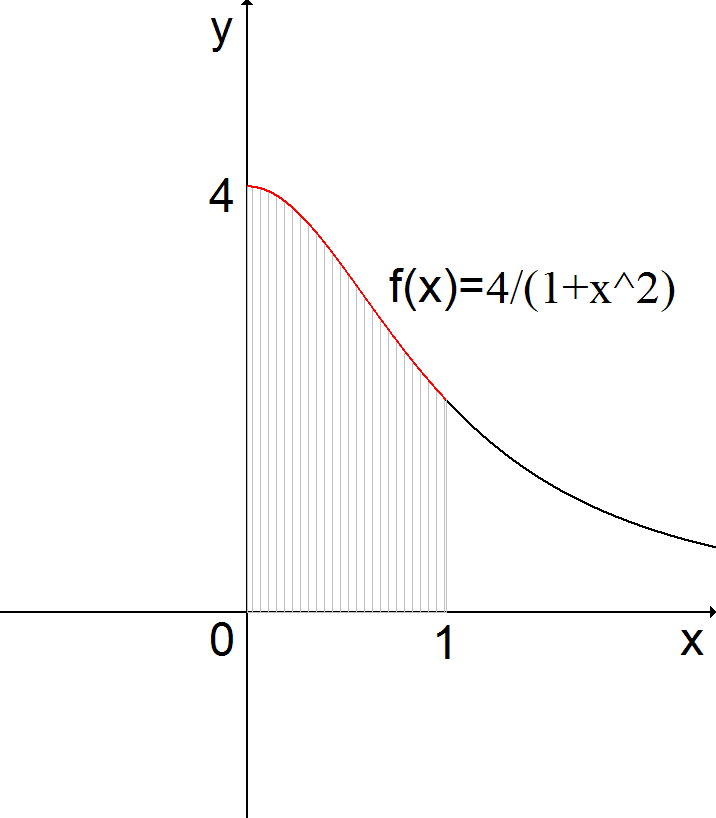
\includegraphics[width=0.5\textwidth]{img/piFunction.png}
     \end{center}
\end{column}

\begin{column}{0.5\textwidth}  %%<--- here
    \begin{center}
     
\includegraphics[width=0.5\textwidth]{img/formula_a.png}
     \end{center}
     \vspace{5mm}
     \begin{center}
     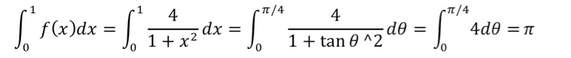
\includegraphics[width=1.0\textwidth]{img/formula_b.png}
     \end{center}
      \vspace{5mm}
     \begin{center}
     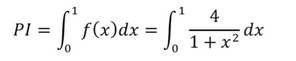
\includegraphics[width=0.5\textwidth]{img/formula_c.png}
     \end{center}
\end{column}
\end{columns}




\end{frame}

\begin{frame}[fragile]{Collective communication exercise}
\vspace{5mm}
\begin{itemize}
\item Calculating pi using trapezoidal rule:
    \begin{itemize}
    \item Divide interval up into subintervals.
    \item Assign subintervals to processes
    \item Each process calculates partial sum
    \item Add all the partial sums together to get pi.
    \end{itemize}
\vspace{5mm}    
\item Subinterval information:
    \begin{itemize}
    \item Width of each subinterval (w) will be 1/n
    \item Distance d(i) of segment "i" from the origin will be "i*w"
    \item Height of segment "i" will be f(i)
    \end{itemize}
\end{itemize}

\end{frame}

\begin{frame}{Extra exercise}
\begin{itemize}
\item Try to implement a matrix-matrix multiplication algorithm using MPI.
\begin{enumerate}
    \item Do it using only MPI\_Send and MPI\_Recv.
    \item Do it using MPI collectives (hint: MPI\_Scatter, MPI\_Gather may be useful)
\end{enumerate}
\end{itemize}
\vspace{5mm}    
\begin{center}
     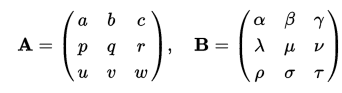
\includegraphics[width=0.4\textwidth]{img/mm_1.png}
\end{center}

\begin{center}
     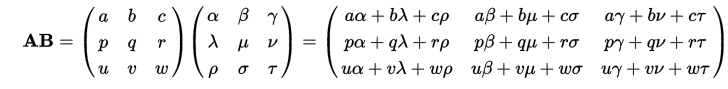
\includegraphics[width=0.8\textwidth]{img/mm_2.png}
\end{center}

\end{frame}


\begin{frame}[fragile]{Timing parallel execution}

\begin{itemize}
\item Main goal: improving performance. 
\item Elapsed or wall time is used to measure speedup and efficiency, not CPU time. 
\item MPI provides timing functions

    \begin{lstlisting}
    double start, finish;
    
    start = MPI_Wtime();
            .
            .
    /*Code being timed*/
            .
            .
    finish = MPI_Wtime();
    printf("Elapsed time:  %f seconds\n",finish-start);
    \end{lstlisting}

\item Minimize communication, maximize computation! 
\end{itemize}

\end{frame}

\section{Concluding Remarks}

\begin{frame}{Concluding Remarks}

\begin{itemize}
\item MPI is an industry standard model for parallel programming.
    \begin{itemize}
    \item Gives the programmer great parallelism power.
    \item The programmer has to explictly indicate and control data movement and synchronization. 
    \end{itemize}
\item Performance usually sensitive to assignment of tasks to processors due to concurrency, workload balance, communication patterns, and more.
\item Special caution must be taken to avoid unsafe communications and possible deadlocks. 
\item Overlapping communication and computation is key to reducing execution times and improving performance. 
\item Not all problems are suitable for parallelization using the message-passing model.
\end{itemize}

\end{frame}

\begin{frame}{To Infinity and Beyond}

\begin{itemize}
\vspace{10mm}
\item Hybrid applications: MPI + X (OpenMP, PThreads, ACC)
\item One-sided communications: operations that do not require both ends to synchronize during communication.
\item Non-blocking collectives.
\item Communicators and topologies: mapping virtual topologies to underlying physical structure. 
\item Neighborhood collectives.
\end{itemize}

\end{frame}

